
\section{Architectural Design Pattern}

VTK is an object-oriented system with carefully controlled access of data members which are either protected or private.  In general, the architecture of the toolkit relies on a Pipe-And-Filter architectural design pattern, yet various consistencies have to be managed to make this architectural decision successful such as:

\begin{figure*}[h!]
    \centering
    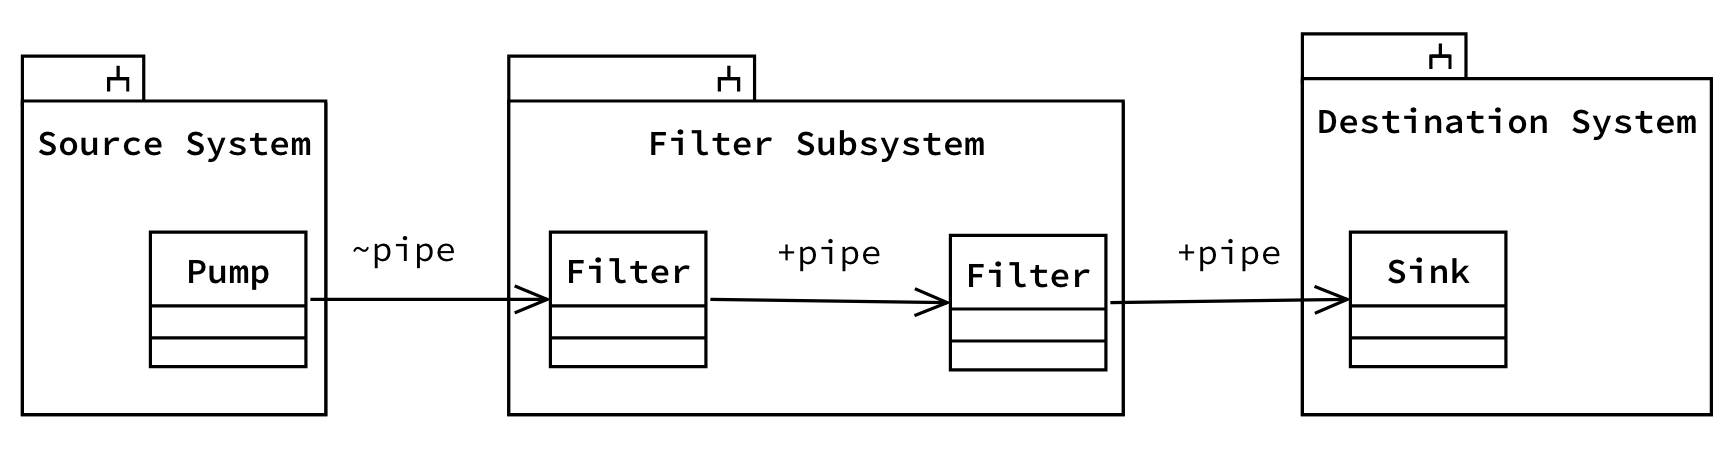
\includegraphics[width=15cm]{diagrams/filter-pipe.png}
    \caption{Pipe-And-Filter Pattern}
    \label{fig::design::pattern}
\end{figure*}


\begin{itemize}

    \item Using condensed means of representing and managing data; arrays (e.g. \code{vtkFloatArray}) are usually contiguous pieces of information. This design has purposely adopted because it is much more efficient to allocate and deallocate memory in large contiguous chunks and also because it is easier to send through pipes data uniformly organised \cite{aosabook}.
    
    \item VTK has a comprehensive collection of convenience methods for writing and reading information, including methods for fast access, and methods that automatically allocate memory as needed when adding more data \cite{aosabook}.
	
    \item Restricted access to class attributes through setters and getters; most objects in the toolkit require input/output references to connect inside the pipeline or interchange; this method allows for more flexibility when constructing the data flow pipe.

    \item VTK uses the PIMPL design pattern (pointer to implementation) to hide complexities of a template implementation; the solution is generally used in C++ code bases to improve the compilation time.  In  PIMPL, the developer separates the implementation (algorithm/complexity) from a given class into a simple structure, then the structure is uniquely referenced inside our class, we can later inject the algorithm as a dependency with DI. 
    
\end{itemize}
 
	
VTK consists of several major subsystems such as data management, web environment, interactive data subsystem \cite{aosabook}, yet most associated with visualisation packages is the pipeline architecture. 

In concept, the pipeline architecture consists of three basic classes of objects: objects to represent data (the \code{vtkDataObjects} discussed above), objects to process, transform, filter or map data objects from one form into another (\code{vtkAlgorithm}); and objects to execute a pipeline (\code{vtkExecutive}) which controls a connected graph of interleaved data and process objects \cite{aosabook} (i.e., the pipeline). Figure 24.3 depicts a typical pipeline.


\subsection{Components}

The pipeline architecture consists of three types of components: 

\begin{itemize}
    \item \textbf{data components} which represent the data such as \code{vtkDataObject} 
    \item \textbf{process components} which transform, filter or map a set of data objects from one state to another, e.g. \code{vtkAlgorithm} 
    \item \textbf{executive components} which manage and execute the pipeline (e.g. \code{vtkExecutive}); those objects control the connected graph and the data objects through the process components   
\end{itemize}

While the description of those components is oversimplified, due to the nature of the project, some complications occur for every type of component \cite{git}.

The representation of data components can become complicated; some algorithms/processes require sets of hierarchies or grouping of data, which results in a non-trivial iterative or recursive execution.  In other cases, parallel processing (shared-memory scalars or distributed data sets) require partitioning of our input data into smaller pieces, which may overlap to compute the final result.

\begin{figure}[h]
    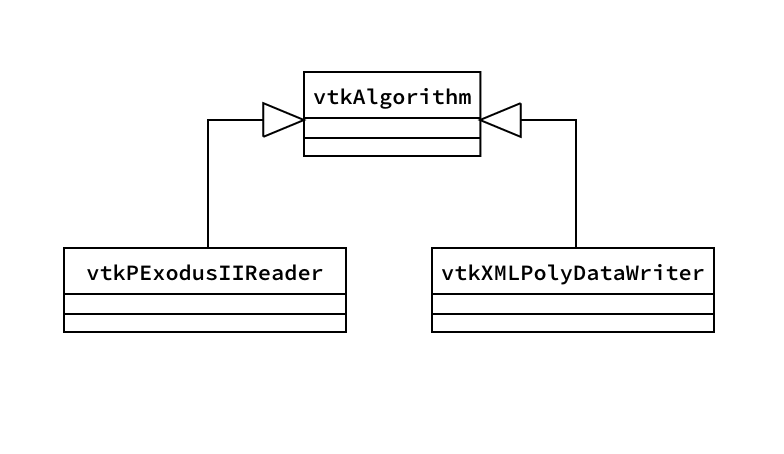
\includegraphics[width=8cm]{diagrams/alg.png}
    \caption{vtkAlgorithm Executive Component}
    \label{fig::executive}
\end{figure}

The process components also add their complexity \cite{git}; some algorithms may vary in the number of inputs required or may produce multiple outputs of different types. Algorithms can operate locally on data or with global information. 

Finally, the executive components depend on their particular execution strategy. In some cases, they may cache intermediate results between filters, reducing the number of recomputations performed when something in the pipeline changes. 

\subsection{Relationships \& Roles}


\begin{figure*}[h!]
    \centering
    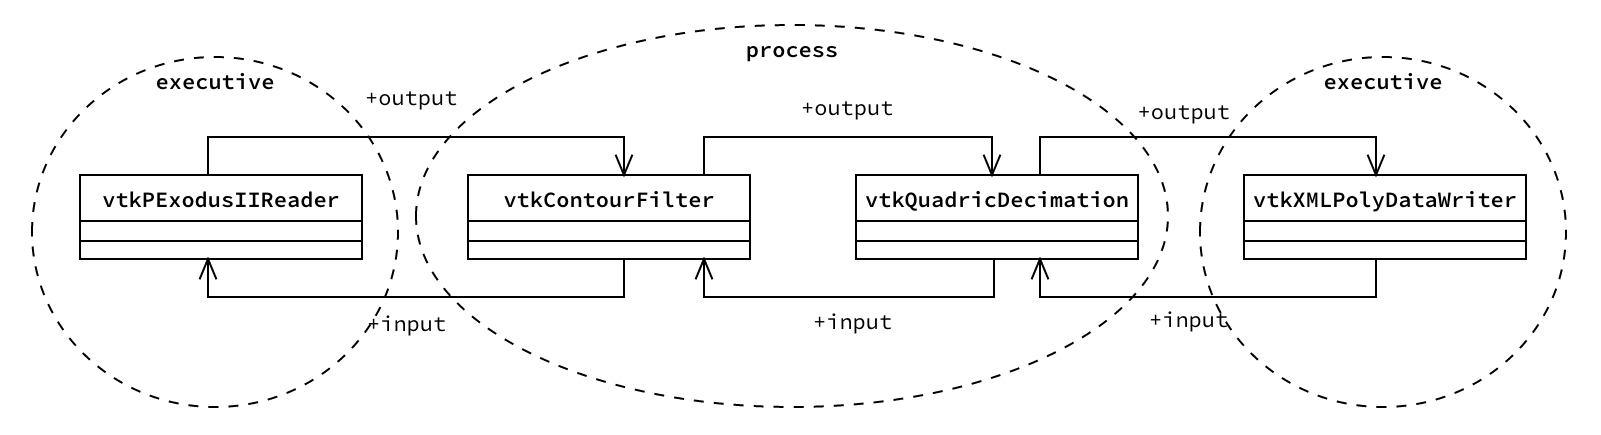
\includegraphics[width=15cm]{diagrams/process.png}
    \caption{Pipeline Infrastructure}
    \label{fig::pipe}
\end{figure*}

Because each process component provides data for the next process component or actor in the pipe chain,  they treat their data components as immutable objects, when producing their output. Various process components can be linked together and composed into filters to transform the information \cite{aosabook}. This composition creates the pipeline/chain process, which ends with an actor.

The following code example illustrates the relationship between our components:

\writecode{c++}
    {code/example.cpp}
    {Pipeline Example Usage}
\label{fig::pipeline::example::code}

The writer reduces the result of the pipeline to a data file because the output of the pipe is redirected as an input connection to our writer.  The pipe consists of two filters, process components which computes data components provided by a given source (a file reader).

The execution objects manage the data flow when the writer demands data during the execution of its write function. For example, if the value of the target reduction is changed to another value, the executing object will notify the process component to reevaluate its output and will use the cached output value from the first process component in the pipe as an input for this reevaluation \cite{aosabook}.

The pipeline execution mechanism is demand driven; \code{VTK} evaluates the output of the pipe only when the sink uses its data components. The request for data components will propagate through the pipe/chain of process components until it reaches the source (pump), in this case, the file reader. 

By default, each process component caches its output to avoid unnecessary executions in the future; by adding a time stamp to the result (e.g. \code{ComputeTime}) \cite{aosabook}.

\subsection{Quality Properties}

In terms of \textbf{testability}, the system is easy to test in isolation because the programmer has to compare the output of a process component with the expected output; thus, an assertion can be made with ease. For integration testing, VTK provides "fake" execution processes to simulate the normal execution of our pipeline.

Ensuring the \textbf{scalability} of VTK is challenging due to its architecture; it is difficult to scale individual components of the pipeline. The environment of VTK provides high \textbf{performance} compute-intensive algorithms and \textbf{flexibility} to its users.